\chapter{Methodology}\label{ch:methodology}
% Description of what has been done: a clear description of any activities performed in the project, such as data collection, implementation, data analysis, set up of any experiments, etc. 
% Containing a comprehensive description of the design chosen, how it addresses the problem, and why it is designed the way it is.

%-----------------------------------------
\section{Overview}
Several possible approaches can be taken to achieve this paper's research aims. Current \acrshort{sota} transformer models provide several methods. Firstly, a pre-trained model (such as \acrshort{bart}, T5 or \acrshort{gpt}) can be fine-tuned using \acrfull{mlm} on a specific document. Alternatively, a fully fine-tuned model can be used and simply fed the most relevant paragraphs from the `knowledge' base. A third and final model is a combination of the other two approaches: a pre-trained model can be fine-tuned for general question-answering from a context, such that questions are posed to the model with the most relevant paragraphs from the `knowledge' base included as context.

`Knowledge' in this context is used to refer to the information that the model aims to learn and will be used like this henceforth. This `knowledge' can be in the form of websites, \acrshort{pdf}s (e.g. textbooks), and other supporting documents used by a module. Pre-training a model provides more flexibility and opportunity for the model to become very good at this specific task, but is much more resource-intensive, may be difficult to achieve high-quality results, and can be less scale-able. I will begin by discussing the methodology behind creating the `knowledge' base used by the transformer models, and then proceed to outline the different models which this paper will compare.

% the pre-trained model or pass the information into the model during the question-asking stage, using a fine-tuned model.

% \begin{enumerate}
%     \item 
%     \item Custom question generation: a laborious approach where the module convenor is required to create a set of questions and answers that are used to train the model
%     \item Document store: Splitting the `knowledge' into different sections and finding relevant paragraphs to a student's query (using cosine similarity). The relevant paragraphs can be fed into a fully fine-tuned model (e.g. \acrshort{gpt}-3.5 Turbo)
%     \item Question-answering fine-tuning: Taking a pretrained model (e.g. T5 or \acrshort{bart}) and fine-tuning this for question-answering. Then paragraphs which are relevant to the query can be fed into the model which extracts an answer. 
% \end{enumerate}
\subsection{Knowledge}\label{sec:methodology_knowledge}
In order to encapsulate the `knowledge' any chatbot should aim to contain, relevant documents were obtained from the University of Nottingham's COMP-2032 Computer Vision module. These included textbooks, lecture notes, and lecture transcripts. Due to the lecture notes containing only key headline information which was then discussed in audio format, lecture notes were not used to fine-tune the model. Furthermore, the transcripts were of poor quality and contained mistakes which could cause any model to perform badly. Subsequently, only textbooks were used to form the `knowledge' base, because they were of high-quality and were around 500-1000 pages long. The two textbooks used to form the `knowledge' base were `\textit{Digital Image Processing textbook}' \citep{gonzalez2018digital} and `\textit{Fundamentals of Digital Image Processing textboo}k' \citep{solomon2010fundamentals}.

PDF textbooks were parsed using Python's \texttt{Fitz} package (from \texttt{PyMuPDF}), with the text extracted using the package's \textit{blocks} functionality, meaning that text was extracted line-by-line, or by paragraph depending on the context. This text was cleaned to remove websites, and then each block of text was merged with the next until the token limit (800) was reached. There is a trade-off between merging potentially irrelevant content, having large contexts to provide the model with as much background information as possible, and having section lengths that can be processed by multiple models. Additionally, the tokeniser used to determine the number of tokens per section was the `all-mpnet-base-v2' model \citep{huggingface_tokeniser_model}, as it typically produced higher token counts than \acrshort{gpt} and T5, meaning that sections would never be larger than other models can handle.

Similar functionality was implemented for Wikipedia pages, to allow lecturers to provide specific pages that are relevant to a course. These pages are split into sections according to their headers and then split again using a delimiter if the section contained more than 800 tokens (as above). None of the models in this paper use Wikipedia, but the code has been included for completeness and future development.

%  ADD REFERENCES FOR THE CODE I USED FROM THE OPENAI COOKBOOK
\subsection{Setup} \label{sec:design_setup}
All models below were fine-tuned and run using Google Colab \citep{Bisong2019}. Access to \acrlong{gpu}s (\acrshort{gpu}s) was kindly provided by the University of Nottingham, but the vast size of the models in comparison to the quality of \acrshort{gpu}s available meant that training could take up to 10 hours or more to complete and required more \acrshort{ram} than was available. Colab Pro provided access to Google's A100 \acrshort{gpu} was available with 40GB \acrshort{gpu} \acrshort{ram}, 80GB \acrshort{cpu} \acrshort{ram}, and over 200GB of disk space. A virtual environment with the following deep learning packages was used: \emoji{hugging-face} \texttt{Transformers} (4.31.0), \texttt{PyTorch} (2.0.1+cu118), \texttt{Datasets} (2.13.1), and \texttt{Tokenizers} (0.13.3). The \emoji{hugging-face} \texttt{Transformers} library (specifically the \texttt{Seq2SeqTrainer} class) was directly used to fine-tune the models \citep{wolf2020huggingfaces}. \acrshort{gpt}'s embedding model used the \texttt{Tiktoken} package (0.4.0) which requires Python >=3.8. Finally, all training, shuffling, and processes were conducted with a seed value of 9 to ensure reproducibility.

%-----------------------------------------
\section{Masked Language Modelling}\label{sec:methodology_mlm}
% Could work, although it would not be trained in question-answering.
The simplest model produced in this paper is a fine-tuned version of a pre-trained model (\acrshort{gpt}). The chatbot is fine-tuned to the module's domain (Computer Vision) by using \acrfull{mlm}. By randomly `hiding' (masking) a proportion of the tokens within the training data (e.g. a textbook), the model is trained to predict their value. This is discussed fully in Section \ref{sec:background_implementations}.

\subsection{Training}
This model was trained using the Digital Image Processing textbook \citep{gonzalez2018digital} and validation metrics were computed using the Fundamentals of Digital Image Processing textbook \citep{solomon2010fundamentals}. Both textbooks were imported into the `knowledge' base as described in Section \ref{sec:methodology_knowledge} and then exported into a \texttt{txt} file, with excess line breaks removed. The text was then additionally split into blocks of 512 tokens, using the \acrshort{gpt} tokeniser. The model was trained with a batch size of 16 (due to \acrshort{ram} constraints) for 20 epochs. Regularisation was used to prevent overfitting, a with weight decay value of 0.01 and dropout of 0.6. Training used a learning rate of 3e-5, and took around 30 minutes to complete as the use of an early stopping callback (with a patience of 3 and a threshold of 0.05 for the validation loss) meant that the model finished training after almost 7 epochs. % This is a limitation of the model

\subsection{Evaluation Metrics}
The main metric used to evaluate this model was perplexity, which is defined as the exponent of the cross-entropy validation loss of the model. Perplexity values can be any number above 1, and most language models aim to have perplexity values in the single digits. This is because a lower perplexity indicates that the model is more confident and accurate in predicting the next word, as it better understands the domain and context of the text. This is the most important factor in determining whether the model has accurately `learnt' sufficient information to be able to respond to queries and provide accurate responses. 

% WHY 512 TOKENS??

%-----------------------------------------
% \section{Custom question creation}
% \acrfull{mlm} excels at training a model to learn information about a specific domain. However, there are several potential issues with this model. Firstly, the model is not fine-tuned specifically on \acrshort{qa}, which means that it may lack the ability to properly identify and answer questions. Secondly, without a lot of high quality textual training data, the model could produce responses which sound realistic due to its pretraining on public information.

% Therefore, an alternative model is to produce a set of custom questions and answer pairs based on the module information. These can be used to fine-tune the model so that it learns to identify and respond to questions in an appropriate manner. 72 questions and corresponding answers were manually created and used to train the model. 


% Put this in the results section?
% Unlikely to know knowledge beyond what it has been fed
% Could still use `knowledge' from outside the custom question creation (prove this in the results section)
% Time consuming and not scalable

%-----------------------------------------
\section{Document Store With \acrshort{gpt}-3.5 Turbo}
The second approach used by this paper is the document store approach, combined with a fully fine-tuned \acrshort{gpt} model. Given a set of documents (word documents, \acrshort{pdf}s, Wikipedia pages), this framework chunks them into sections which contain sufficient context but are short enough to be processed by the model (and not use an inefficient or excessive number of tokens). These sections are stored in a data frame, along with the document name/section header, from which section embeddings are created.

The embedding model can be flexible, provided the same embedding model is used to also embed the student's question. GPT's embedding model is faster and can process much longer contexts, but these longer contexts cannot often be handled by other models (e.g. T5). Additionally, it has a small financial cost associated (Section \ref{sec:results_costs}). The \acrshort{gpt} embedding model was used during model testing, but functionality for the use of an open-source alternative such as the `all-mpnet-base-v2' model \citep{huggingface_tokeniser_model} was also implemented.

Once the embedding model has been chosen, the sections of `knowledge' can be embedded. The user's question is then also embedded, with its cosine similarity between each section of `knowledge' used to determine the top (n) relevant sections. These sections are fed into the \acrshort{ai} model, along with the student's question, and it provides a response. If the model can't find an answer in the context provided, it responds appropriately. This framework is shown in Figure \ref{fig:initial_framework}.

\begin{figure}[h!]
    \centering
    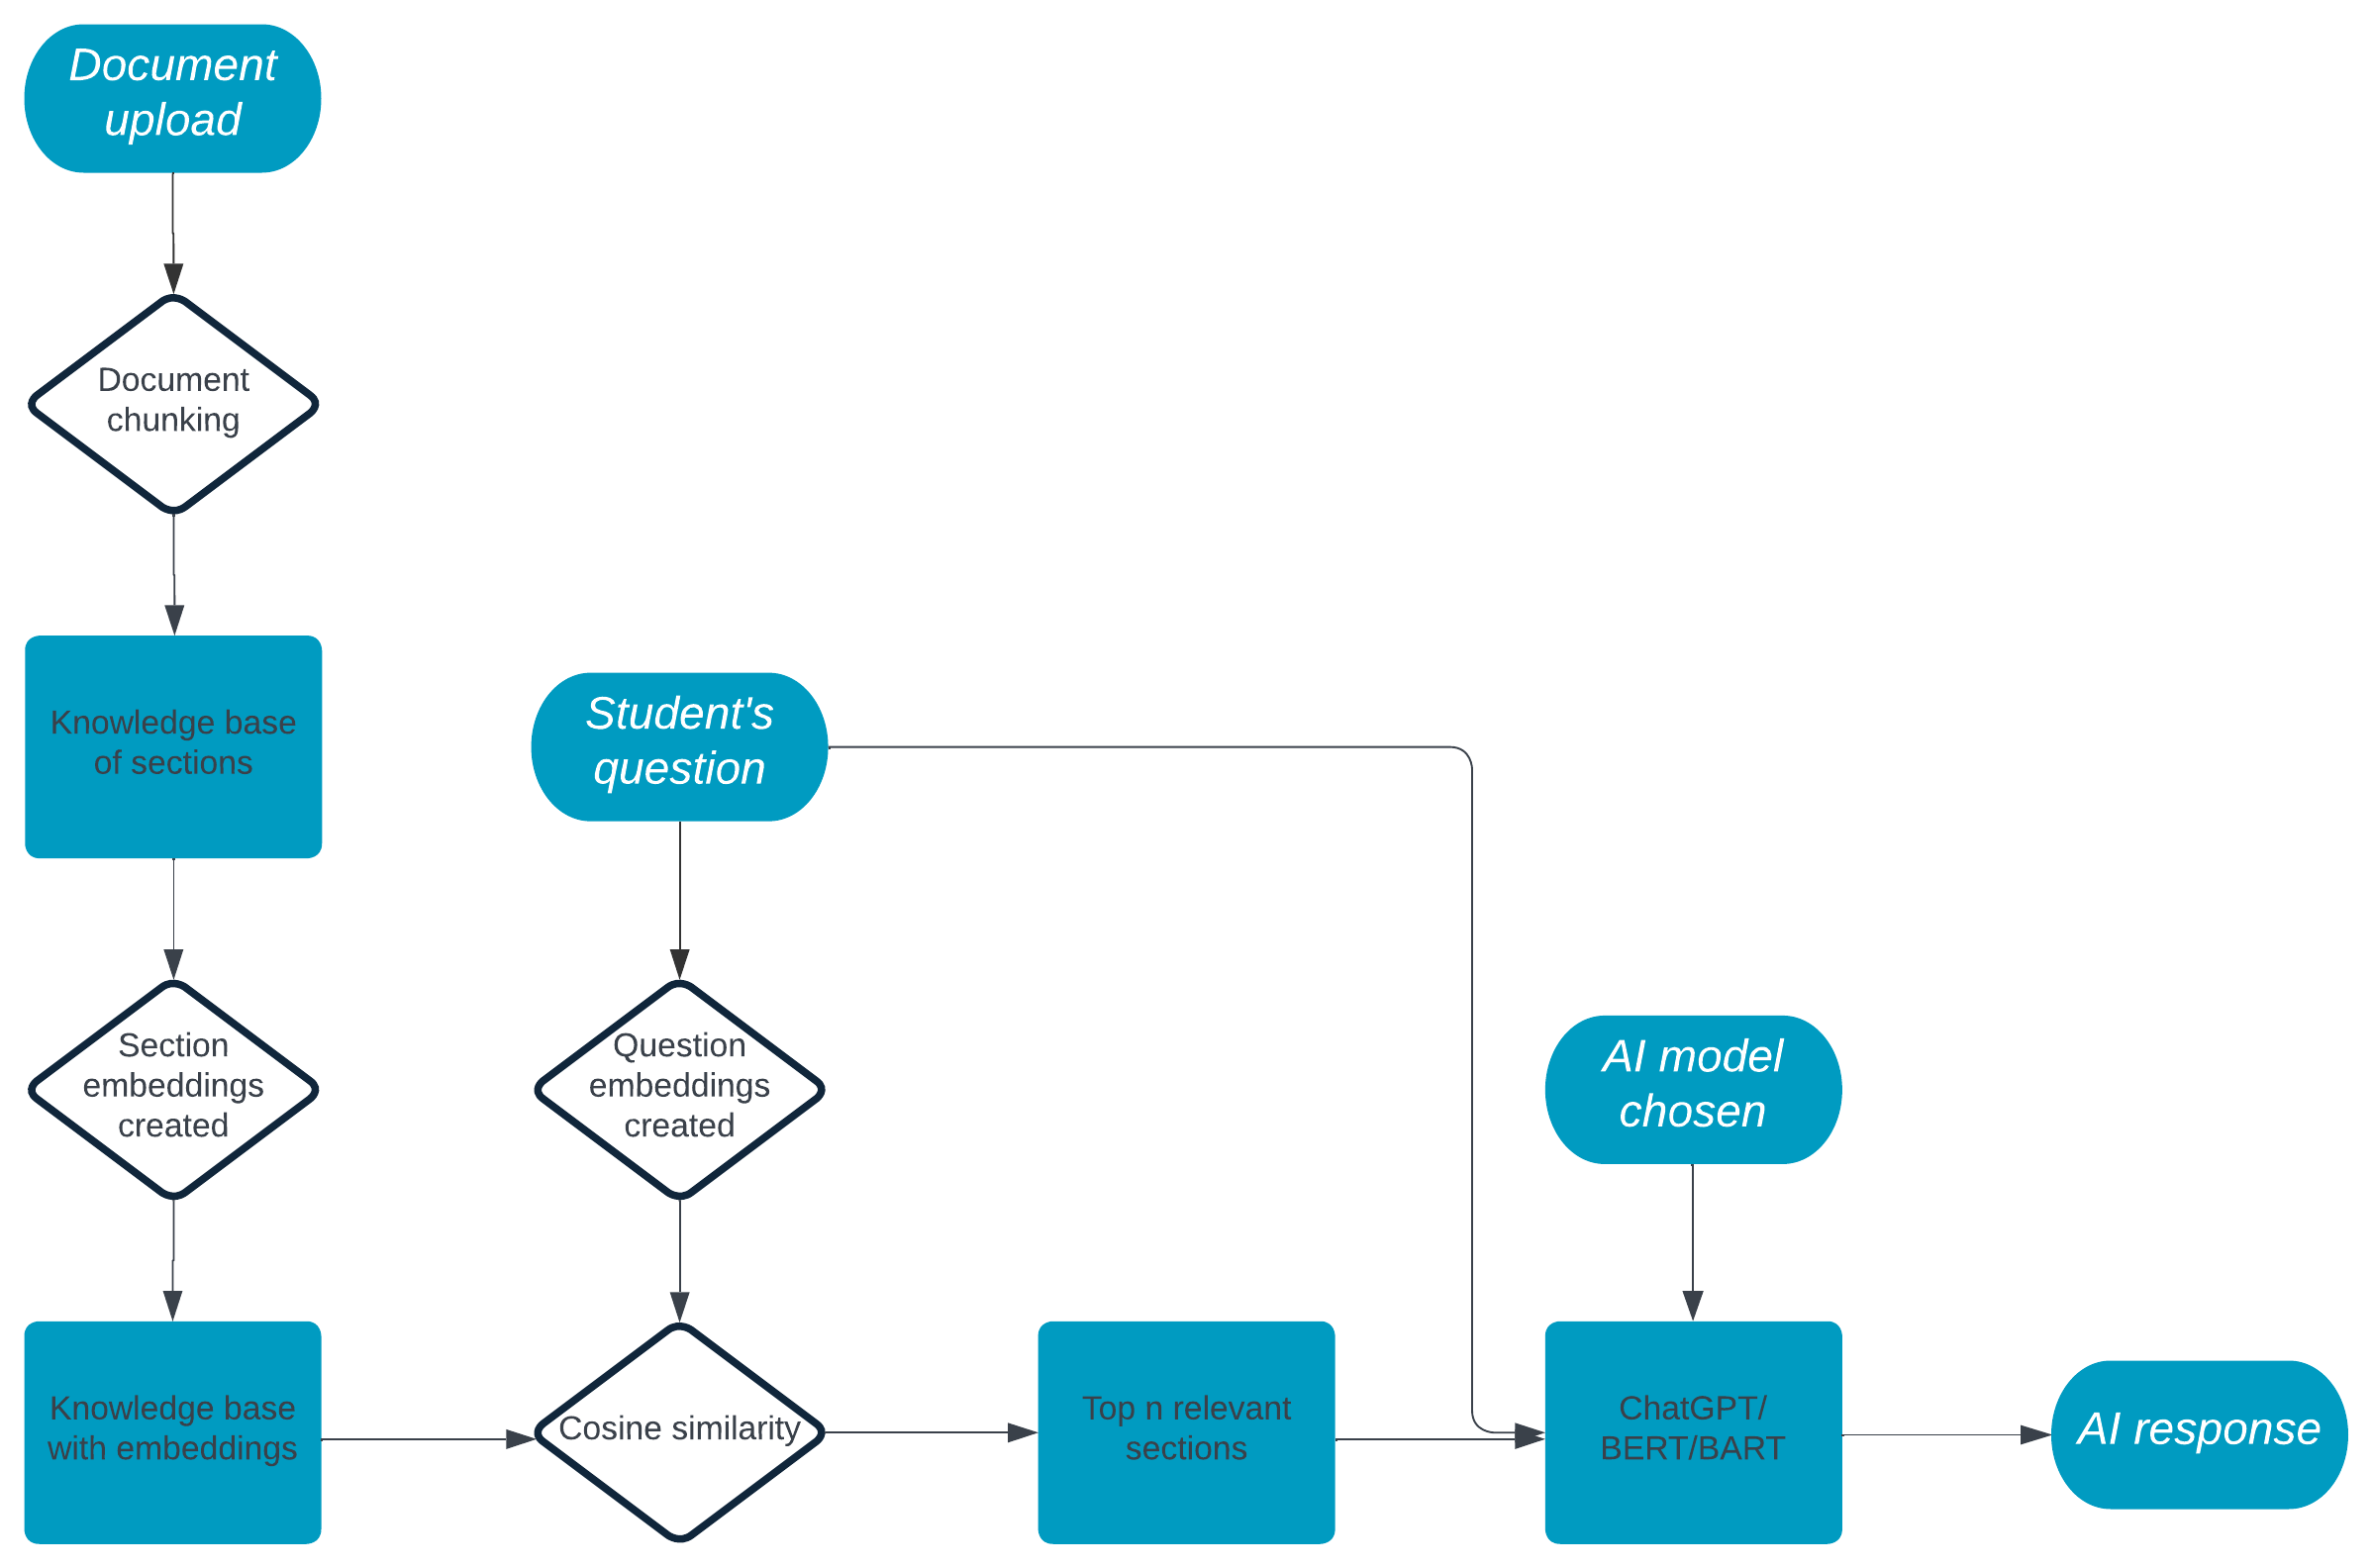
\includegraphics[width=0.8\textwidth]{images/framework.png}
    \caption{Document Store With \acrshort{ai} Chatbot Framework}
    \label{fig:initial_framework}
\end{figure}

\subsection{Implementation}
The document store/`knowledge' base for this model used the two \acrshort{pdf} textbooks outlined in Section \ref{sec:methodology_knowledge}. The top 5 sections were fed into \acrshort{gpt}-3.5 Turbo using OpenAI's \acrshort{api}, along with an instruction to:
\begin{itquote}
    Use the below article on Computer Vision, to answer the subsequent question. If the answer cannot be found in the article, write: I could not find an answer in the text I've been provided, sorry! Please try again.". If you are asked to produce any code, then decline the request and write ``Sorry but I'm not allowed to do your assignments for you!".
\end{itquote}
There was also a combined token limit of 3596, due to the \acrshort{gpt} \acrshort{api} token limit of 4096 being reduced by 500 tokens to allow for a response. This approach benefits from being efficient and less resource-intensive, as it uses the existing fine-tuned \acrshort{gpt} model. Only the top 5 sections of knowledge were provided to the model, provided they had a cosine similarity of greater than 0.5. The limitations help to minimise any token wastage when using the \acrshort{api}.

\subsection{Potential Drawbacks}
A key drawback of this model is the large cost. While the costs associated with this model will be discussed in Section \ref{sec:results_costs}, they are large and may be difficult for teaching departments to justify, given that ChatGPT is currently free. Additionally, the model would always be dependent on OpenAI's support for the \acrshort{api}, along with its availability and stability. The reliability of the \acrshort{api} is beyond the control and scope of this paper but could harm the feasibility of this setup in practice.


%-----------------------------------------
\section{Document Store With Fine-Tuned T5}\label{sec:methodology_t5}
The third model considered by this paper is a combination of the above two models. The challenge is to achieve the accuracy of a fully fine-tuned model (such as \acrshort{gpt}-3.5 Turbo) at a fraction of the cost. The framework in Figure \ref{fig:initial_framework} can be adapted to use any relevant \acrshort{ai} model. For this model, only contexts with a cosine similarity of above 0.7 were provided as an input, to assist with detecting unanswerable questions. If the model is fine-tuned to answer a question using a provided context, it can excel at extracting answers and recognising when an answer cannot be found. This can be achieved by adapting an innovative method of training which is typically used for article summarisation tasks, involving sequence-to-sequence training. 

\subsection{Dataset}
Training the model for question-answering used Google's Natural Questions dataset \citep{NQdataset}. It is the only dataset known to contain naturally phrased questions with answers in natural language. While the answers are extractive (i.e. directly contained within the context provided), they are long-form answers which can be used to fine-tune a model to write natural-sounding answers.

This dataset consists of 307,373 training examples and 7,830 examples for validation. Each example contains a question related to a specific Wikipedia page, which was given in both \acrshort{html} and tokenised form. Both a short answer (at most five tokens) and a long answer were available, with some answers being descriptive and therefore only having a long answer.

\subsection{Pre-Processing}
The dataset requires 154GB of disk space and so only the relevant information was maintained. To clean and reduce the disk size of the dataset, only the question, long answer, and page content in tokenised form were retained. Answers were cleaned to remove any unnecessary whitespace, and the tokenised page content was cleaned of any references (e.g. [2]).

Additionally, only examples which have answers contained within a \texttt{<P>} tag were kept (approximately 72.9\%), as the main aim of the model is to provide textual answers rather than use tables and lists. Answers using the following \acrshort{html} tags were therefore removed: \texttt{<table>}, \texttt{<tr>}, \texttt{<th>}, \texttt{<td>}, \texttt{<ul>}, \texttt{<li>}, \texttt{<dl>}, \texttt{<dd>}, \texttt{<ol>}, \texttt{<dt>}. Furthermore, examples with a particularly short context (<100 tokens) or more tokens than 1024 were removed. This upper limit was chosen because most models cannot process more than 1024 tokens. The model used for fine-tuning in this paper (T5, see section \ref{sec:methodology_qa_training}) can process more than 1024 tokens, but there is an efficiency/memory trade-off.

One drawback of the dataset is that Wikipedia articles typically start with a summary paragraph which is unrealistic for this use case. Therefore, any model may be skewed to incorrectly return the first sentence as the answer. To combat this, any examples where the answer is simply the first line or paragraph were also removed (approximately 16\%).

Additionally, the above pre-processing results in a very high proportion of unanswerable questions relative to answerable ones. As a result of this, the number of unanswerable questions was reduced to only 30\% of the training and test sizes. This was achieved by removing a random sample of the unanswerable questions. Finally, the combined dataset was split into a training and validation set using an 80-20 ratio, with 13,595 training examples and 3,400 validation examples. A \texttt{[NO\_ANS]} token was used to denote an unanswerable question.

\subsection{Data Enhancement}\label{sec:methodology_data_enhancement}
A key limitation of the Natural Questions dataset is that it provides only extractive answers. The answers are a sentence or paragraph of information which can contain irrelevant information to the question. Therefore, fine-tuning a model using this data will not train it to produce succinct summary answers, and it may even struggle to identify correct answers as the training answers can be too large and contain ambiguous content.

To address the issue of poor-quality answers, a one-off enhancement to the dataset was conducted using \acrshort{gpt}-3.5 Turbo. \acrshort{gpt} was provided with each question-answer pair and asked to answer the question by only using the answer provided. The development and implementation of this had a one-off cost of only \$20; however, \acrshort{gpt} was unable to answer 25.6\% of the questions. For example, \acrshort{gpt}-3.5 Turbo was unable to find the answer to the question ``charlie puth we don't talk anymore album" when given the following context:

\begin{itquote}
    ``We Don't Talk Anymore" is a song produced and performed by American singer Charlie Puth from his debut studio album Nine Track Mind (2016). It contains guest vocals from Selena Gomez. Jacob Kasher co-wrote the track with the artists. The song was released on May 24, 2016, as the third and final single from the album. Musically, it is a pop song with tropical-inspired production.
\end{itquote}

The correct answer of ``Nine Track Mind'' was available but not identified; although, this example highlights the necessity to succinctly rewrite answers, as the original answer contains irrelevant information about the type of song and its location on the album.

Therefore, around 1 in 4 question-answer pairs were removed as a result of this process, causing the resulting dataset to contain 10121 training examples and 2484 validation examples. While a reduced dataset is unfortunate, some questions were ambiguous and not necessarily answerable using the context. As such, the process of using \acrshort{gpt}-3.5 Turbo to rewrite answers refined the dataset to only include high-quality examples. After this process, an additional random subset of unanswerable questions was removed to maintain the 30\% percentage of unanswerable questions. This use of \acrshort{gpt}-3.5 Turbo was a one-off requirement and therefore the ongoing use of this dataset has no reliance on the availability of the \acrshort{api}. However, any model trained from this dataset may be limited in its capacity to learn, particularly if the answers are not as high-quality as human-written answers.


\subsection{Data Format}
Each example was manipulated to be in the following format:

\begin{itquote}
    \textbf{Input:} She is a song written by Charles Aznavour and Herbert Kretzmer and released by Aznavour as a single in 1974. ... Elvis Costello recorded a cover version of the song in 1999. This version, produced by Trevor Jones, was featured over the final sequence of the film Notting Hill, and charted throughout Europe. ... The song has been recorded by many different artists over the years. The most notable versions include: </s> who sings the song she from notting hill?
    
    \textbf{Answer:} Elvis Costello recorded a cover version of the song in 1999. This version, produced by Trevor Jones, was featured over the final sequence of the film Notting Hill, and charted throughout Europe.
\end{itquote}

As can be seen above, the answer to each question is contained within the context, meaning that the model is trained to produce answers using the provided context. The input began with the context and was followed by the T5 separator \texttt{</s>} and the question. The target for the model was the encoded form of the long answer. This sequence-to-sequence fine-tuning aims to train T5 to understand the input and question and respond accordingly.

\subsection{Training}\label{sec:methodology_qa_training}
An MT5 (small) model was trained using 22,512 examples, with a learning rate of 1e-3. Regularisation was used to prevent overfitting, with dropout of 0.4 and weight decay of 0.007. The fine-tuning was conducted using a batch size of 16 and gradient accumulation steps of 8 (due to RAM constraints), and almost 10 epochs, during which training took around 3 hours to complete. 
% (see Section \ref{sec:design_setup})

T5 and other \acrlong{sota} models require huge amounts of computing power that were not available for this research. To combat this, gradient accumulation (using steps=4) and gradient checkpointing  (activation checkpointing) were used to reduce RAM, at the expense of training time \citep{chen2016training}. These adaptations cause model gradients to be accumulated over several batches (4) before updating the weights, and for some intermediate activations to be recomputed during the backward pass instead of storing them in memory. While this does not directly affect model accuracy and performance, it can mean that convergence is slower and larger batches lead to different local minima. Overall accuracy should not be significantly affected \citep{gradientAccumulation}. 

\subsection{Evaluation metrics}
Evaluating \acrlong{llm}s is a difficult task due to their complexity, differing model objectives, and different forms of output; there are many facets to evaluate \citep{chang2023survey}. Consequently, a variety of evaluation metrics will be used to evaluate model performance.

The first metric that will be used is the \acrshort{rouge} score \citep{lin-2004-rouge}. \acrshort{rouge} scores compare the n-gram overlap between the generated answer and the target answer, and also for the longest common subsequence. They are adept at measuring how much key information from the target answer is contained in the generated answer. However, there are many drawbacks to \acrshort{rouge} scores, particularly that they are by nature difficult to compare, as the vocabulary and context vary in each application. Furthermore, a `perfect' score of 100 is unlikely and generally unattainable even for humans, as two sentences with the same meaning can be written in different ways, using different words and connectives \citep{schluter-2017-limits}. Typically a score of around 40 is considered reasonable.

The \acrshort{bleu} metric will also be used, which is similar to \acrshort{rouge} but was initially developed for machine translation tasks. The \acrshort{bleu} score compares the precision of n-grams rather than the recall \citep{papineniBleu}, and the limitations discussed for \acrshort{rouge} scores also apply. Additionally, \acrshort{meteor} scores will be used to evaluate the model \citep{banerjeeMeteor}, which are similar but more complex than a \acrshort{rouge} score. A \acrshort{meteor} score also aims to compare the accuracy of the generated answer to the target answer but additionally considers the alignment of words and phrases between the generated answer and the target answer. Neither \acrshort{bleu} nor \acrshort{meteor} scores have an `ideal' target number, but range from 0 to 100, with the original transformer `Attention is All You Need' paper achieving \acrshort{bleu} a score of 28.4 on the \acrshort{wmt} 2014 English-to-German translation task, and 41.8 on the \acrshort{wmt} 2014 English-to-French translation task \cite{vaswani2017attention}.

However, each of the above metrics fails to capture the semantic accuracy of answers. As a result, the cosine similarity will also be used to evaluate the model, which can range from 0 to 1. This metric will enable an evaluation of how accurately the answer encapsulates the target meaning. Furthermore, the model will also be evaluated using the percentage of unanswerable questions which are accurately identified. This will be calculated by taking the proportion of answerable questions which the model responds to by returning the unanswerable token, \texttt{[NO\_ANS]}.

By using a combination of the above metrics, the overall model accuracy and performance, including word overlap, precision, recall, semantic meaning, and unanswerable response accuracy, will be evaluated.